\documentclass{article}
\usepackage[utf8]{inputenc}

\usepackage{float}
\usepackage{natbib}
\usepackage{graphicx}
\usepackage[export]{adjustbox}
\usepackage{multirow}
\usepackage{hyperref}
\usepackage{titlesec}



\begin{document}
\title{COS301 Team Gamma: WebFrontend Team Goals}
\begin{figure}
    \centering
    
\includegraphics[width=\textwidth]{logo.png}
\end{figure}
\date{March 2020}

\maketitle

\section{Introduction}
This document describes the responsibilities and all deliverables for the \\ WebFrontend Team.
\\ \\
Demo \#1 Due Date: Thursday 12 March 20:00
\newpage

\section{Organisation}
\subsection{ClickUP}
You need to elect a team leader if you have not done so already. Work together with this member to create tasks and sub-tasks for each member in your team on \url{http://clickup.com} (on the COS301 workspace you have been invited to). \\

\begin{figure}[h]
    \centering
    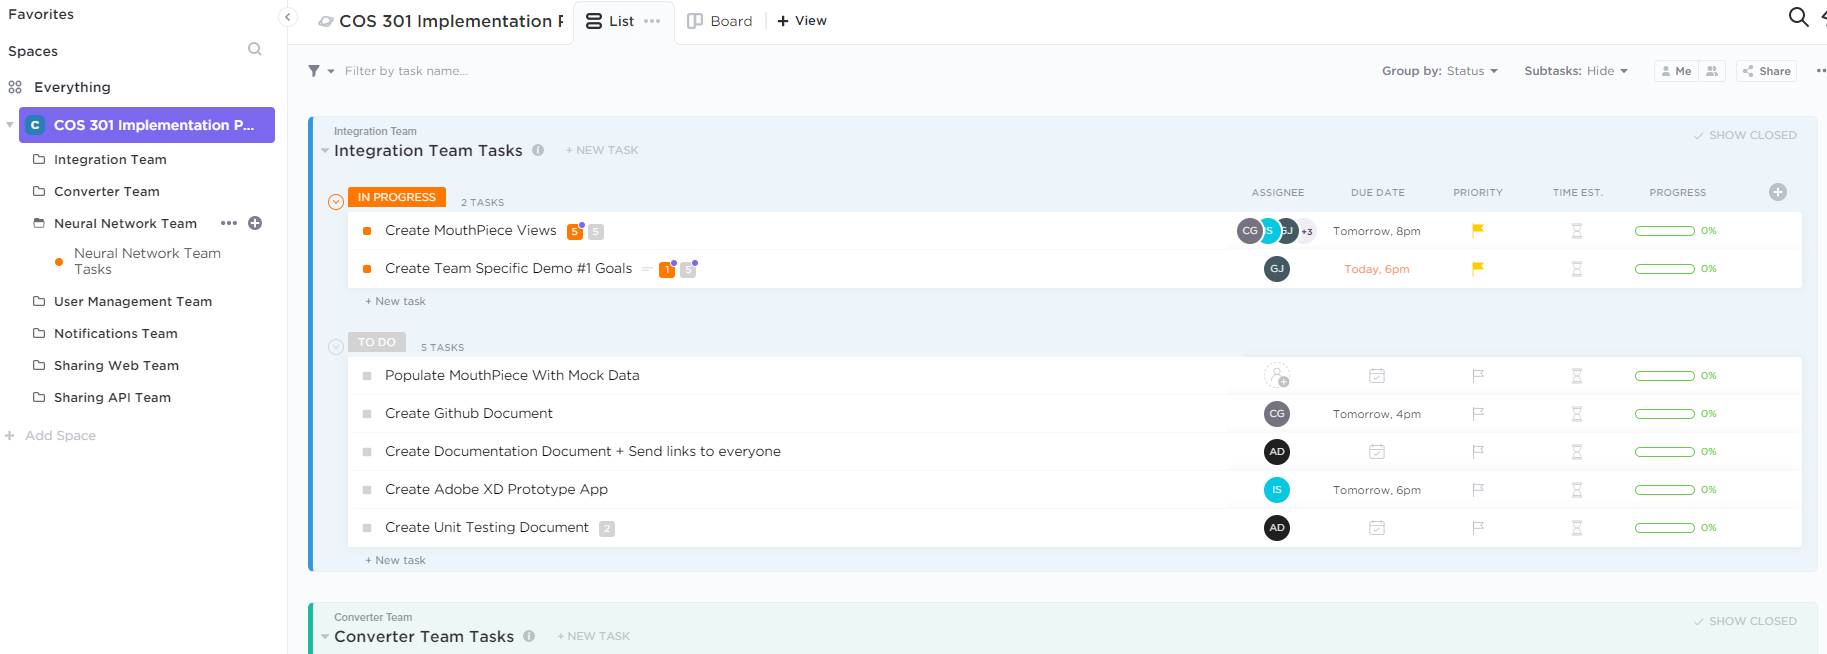
\includegraphics[width=\textwidth]{clickup.png}
\end{figure}

Ensure that you indicate progress and mark tasks as complete. This page will be displayed at the demo.

\subsection{Slack}
Although we have created a WhatsApp group - we do still find it easier for in-group discusions to happen on the slack channels. Simply login to \url{http://cos-301.slack.com}

\newpage

\section{Overall Team Tasks}
These are the tasks to be done by your team for the final product (not specifically Friday's demo).

\begin{itemize}
    \item Deploy a responsive website front-end on an apache server (HTML, CSS, JavaScript)
    \item Communicate with the SharingAPI and UserManagementAPI through HTTP Requests (through JavaScript - JSON format)
    \item Login \& Register page
    \item Update user preferences (when logged in) (Current mouth selected in app, format vs. volume, dark mode etc.) specifics to be determined)
    \item Home : List Mouth Packs (grid interface)
    \item Search and filter Mouth Packs (home page probably)
    \item Upload Mouth Packs (+-12 different images - drag and drop interface preferred)
    \item Download entire mouth pack
    \item Provide a unique URL to a specific mouth pack (e.g. teamgamma.ga/mouthpacks?id=vampire when you click on a design)
    \item Validate user input (e.g. email) on the front end (JS)
    \item Switch between Dark mode and Light mode interface
    \item The website needs have a high visual impact - we are trying to impress
    \item \textbf{REMEMBER: Mouth Pack upload and download needs to be available anonymously - i.e. without login}. In this case you would simply send "ANONYMOUS" as the author to the SharingAPI.
\end{itemize}

\vspace{1cm}

\begin{center}
   \textit{The tasks are always subject to change, but we have tried our utmost best to sketch out the entire project ahead.}
\end{center}

\newpage


\section{Team Tasks for Friday}

\subsection{Documentation}
\textbf{All documentation to be created in Overleaf}

\subsubsection{Web page content}
Create a document with each separate webpage or section as a heading. Describe what will be displayed in each section and via which interface element. \\

You should attach inspiration examples found on other websites, e.g.

\begin{figure}[h]
    \centering
    
\includegraphics[width=\textwidth]{cardui.jpg}
\end{figure}

\newpage
\subsubsection{Frameworks}
You are required to do some research on frameworks that you could implement to assist your \textbf{Overall Team Tasks}. Write a short report on only the frameworks that you are keen to implement. Show its benefits and how you can implement it with the existing technologies. \\

\textbf{Some examples}
\begin{itemize}
    \item \url{https://material.io/develop/web/}
    \item \url{https://getbootstrap.com/}
    \item \url{https://validatejs.org/}
\end{itemize}

\subsection{Hosting Environment}
Your team will already deploy your demo for Friday on the Apache web server. You will demo your FTP setup and showcase the live URL.\\

\textbf{Use the following FTP details:} 

\begin{itemize}
\begin{itemize}
\item Host: ftp.teamgamma.ga
\item Username: webfrontend@teamgamma.ga
\item Password: 2IQve6sgQT
\item Port: 21
\end{itemize}
\end{itemize}

\\

Your FTP login details are rooted in: \url{http://teamgamma.ga/webfrontend/}. i.e. any uploads will be visible on that URL. This will be moved to the root directory on deployment.

\begin{center}
   \textit{If you have any issues with the hosting, or require additional server resources, contact Giovanni (on Slack).}
\end{center}

\newpage

\subsection{Implementation}
\subsubsection{Website Demo}
You are required to build the website front-end and fill it up with mock data. \\

\textbf{More specifically:}
\begin{itemize}
    \item Create all the separate pages as discussed in \textbf{Overall Team Tasks}
    \item Create the navigation and link all the pages
    \item The demo needs to be responsive
    \item Fill up the pages with mock data (fake mouth images, fake profile etc.) One set of mock data is sufficient (one user's logged-in view)
    \item No HTTP requests are required (log-in button redirects to homepage without checking input etc.)
    \item While the design should make an impression, don't worry if it changes down the line
\end{itemize}

\subsubsection{Unit Testing}
Describe how your team will implement unit testing. Better yet - implement it in the Demo where possible.


\end{document}